\documentclass{scrartcl}
\usepackage{hyperref}
\usepackage[utf8]{inputenc}
\usepackage{graphicx}
\graphicspath{{./images/}}
\hypersetup{
    colorlinks=true,
    linkcolor=blue,
    filecolor=magenta,      
    urlcolor=cyan,
}
\urlstyle{same}
\title{Neural Networks in Text Processing}
\subtitle{ Natural Language Processing }
\date{06-01-2020}
\author{Fernando André Bezerra Moura Fernandes - bez0070}

\begin{document}
    \maketitle
    \pagenumbering{gobble}
    \newpage
    \tableofcontents
    \newpage
    \pagenumbering{arabic}
    \section{ Abstract }
    \textbf{Text Processing} allows the automation of creating and manipulating electronic text 
    with numerous modern applications such as grammar and spell checking, text completion,
    plagiarism detection or even chat bots. Thus, the theory behind text processing techniques
    requires a lot of \textbf{algorithmic} and \textbf{data structure} knowledge. \newline
    These techniques allow the development of artificial intelligence applications and with
    normally have to deal with large quantities of strings when analyzing textual documents
    for their different uses. \newline
    One very specific use case of textual analysis is \textbf{Natural Language Processing} 
    which is the one of the two main topics of this document. \newline
    \textbf{Natural Language Processing} is an artificial intelligence field concerned with 
    interactions between computers and a language and (i.e English) and the
    processing of textual data in that language so that the machine can make
    conclusions about that document. \newline
    In order to understand a document written in some language a computer program must first
    pre-process that document so that later it can be modeled in a computable way. 
    Common ways of doing this include:
    \begin{itemize}
        \item \textbf{Tokenizing the document} by breaking down the document's text into 
        different words and representing a document in memory by its words. One example is to
        divide the document by the space character and getting the words that way.
        \item \textbf{Stemming the words} which means to get the base word and removing the 
        derivational affixes.  
        \item \textbf{Lemmatization} by removing the inflectional ending of the words and getting
        the root word ensuring it belongs to that language.
        \item \textbf{N-Grams}. N-grams refer to the process of combining the nearby words 
        together for representation purposes where N represents the number of words to be 
        combined together.
    \end{itemize}
    In order to model a document by its content, first a meaning must be given to the words it
    contains. \newline 
    One way of doing this calculating a \textbf{TF-IDF} value for each word on a
    document, which can be interpreted as its weight. Another way would be calculating
    \textbf{One-Hot Encodings} or \textbf{Word Embeddings} which are other ways 
    of representing words in a document.
    After these transformations the document can be represented in a certain format
    such as a \textbf{Bag of Words}. \newline 
    All these concepts and techniques and much more are used by \textbf{Deep Neural Networks} in 
    the field of Natural Language Processing. \textbf{Neural Networks} are a set of algorithms 
    which are modeled to resemble the way that the human brain works. Deep Neural Networks
    are a subfield of Neural Networks which use multiple layers to progressively extract 
    higher level features of the input they are given. \textbf{DNN} have revolutionized the field
    of Natural Language Processing and are the second main topic of this document. 
    \newpage
    \section{ Introduction }
    Neural networks in the area of computer science are mostly refered to as 
    \textbf{Artificial Neural Networks} and are based on the neural structure of the brain,
    being able to learn to perform tasks such as classification and clustering. \newline
    An ANN consists of a series of nodes, which are interpreted as artificial neurons which
    are part of a directed and weighted graph and can be set on an input layer, 
    output layer, or on the middle hidden processing layer or layers.
    
    \begin{figure}[h!]
        \centering
        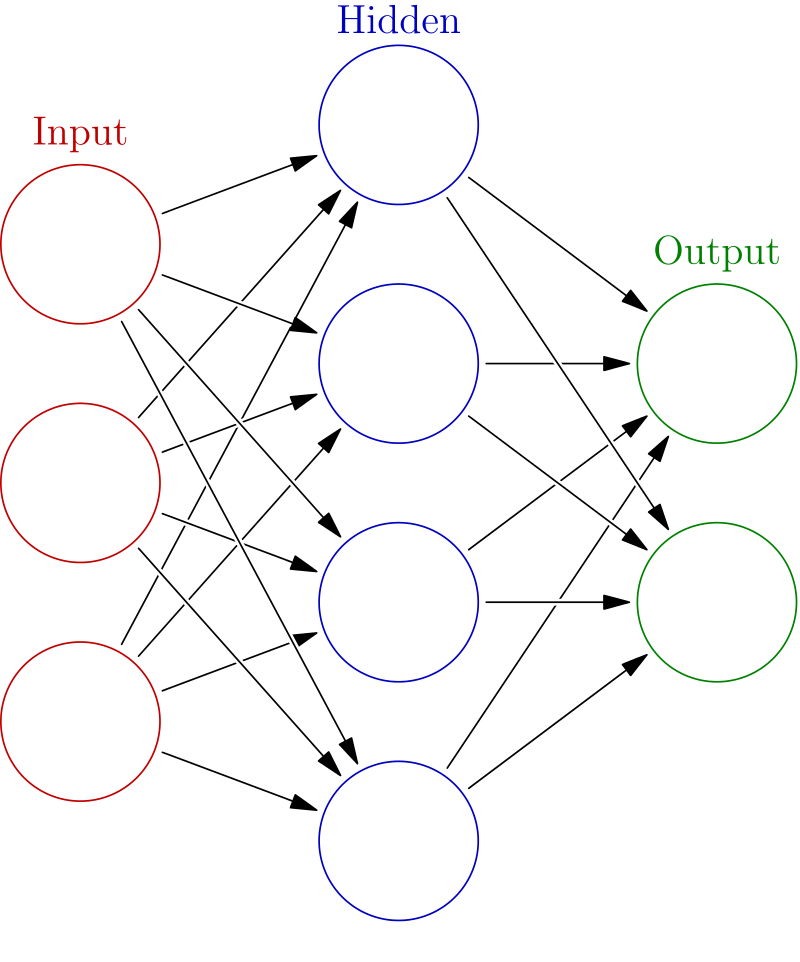
\includegraphics[scale=0.2]{ann.png}
        \caption{A representation of an ANN}
    \end{figure}
    The input layer receives input, parses it and sends information to the hidden layer(s) which
    in turn sends it to the output layer. Every neuron(node) has \textbf{synapses}(input), 
    which they combine with their internal state using an \textbf{activation function} and produce
    an output. The input to a neuron is the output of other neurons or simply another neuron,
    which is computed by a \textbf{propagation function}.
    An ANN also possesses \textbf{hyperparameters} which are parameters who controll the network,
    are set before the learning process and change according via learning. Examples of these 
    parameters include the \textbf{learning rate} or the number of hidden layers and can depend
    on other hyperparameters. \newline
    The ANN consumes a dataset, considering it as a sample observation and uses one part of 
    the dataset(train) to be trained and to learn, varying its hyperparameters and another part 
    (test) to check its accuracy. 
    \textbf{Learning} involves adjusting the weights of the network 
    to decrease an error rate. Usually this \textbf{error rate} is divided among the connections and 
    \textbf{backpropagation} is used to adjust the connection weights. Backpropagation is a method
    who calculates the \textbf{gradient} of the \textbf{cost function}(which measures the performance
    of the ANN regarding its test set) and then the weight updates are often performed using
    \textbf{stochastic gradient descent} or other methods.
    Depending on their internal organization, or the way they change their weights there are many
    different types of ANN, and throughout the rest of this research document, their uses on
    Natural Language Processing will be described.
    \section{ Deep Learning on Natural Language Processing }
    Depending on the NLP task at hand we can use different artificial neural network models and
    achieve different results.
    First we must discuss to how features in a document should be represented. \newline
    Generally speaking, in NLP the sparse-input encodes features such as words
    or part-of-speech tags. The initial task is to parse this input into a neural-network
    base model and start representing each feature as a \textbf{dense vector}. 
    Each feature is \textbf{embedded} into a dimensional space, and represented as a vector in 
    that space, and is treated as a model parameter which needs to be trained together 
    with other components of the network.
    One benefit of using dense and low-dimensional vectors is computational since
    the majority of neural network toolkits do not play well with very high-dimensional, sparse  
    vectors. The other benefit of the dense representations is in generalization power because 
    as some features may provide similar clues, it is worthwhile to provide a representation that
    is able to capture these similarities. \newline
    In cases where we have relatively few distinct features in the category, and we believe
    there are no correlations between the different features,
    we may use the one-hot representation vectors.
    There is also another problem with features related with the number in which they occur, as 
    in some cases their number is not known in advance. Thus, an unbounded 
    number of features needs to be represented using a fixed size vector. One way of doing this
    is using a \textbf{continuous bag of words}. The traditional bag of words 
    is a way to represent the data in a tabular format with columns representing the 
    total vocabulary of the documents, rows representing a single observation and each cell
    being filled up by the observation frequency.
    The CBOW is very similar to the traditional bag-of-words representation in which
    we discard order information, and works by either summing or averaging the 
    embedding vectors of the corresponding features.
    \begin{equation}
        CBOW(f_1, ...., f_k) = \frac{1}{k} \sum^{k}_{i=1}v(f_i)
    \end{equation}
    

\end{document}